%%%%%%%%%%%%%%%%%%%%%%%%%%%%%%%%%%%%%%%%%%%%%%%%%%%%%%%%%%%%%%%%%%%%%%%%%%%%%%%%
%2345678901234567890123456789012345678901234567890123456789012345678901234567890
%        1         2         3         4         5         6         7         8

\documentclass[letterpaper, 10 pt, conference]{ieeeconf}  % Comment this line out if you need a4paper

%\documentclass[a4paper, 10pt, conference]{ieeeconf}      % Use this line for a4 paper

\IEEEoverridecommandlockouts                              % This command is only needed if 
                                                          % you want to use the \thanks command

\overrideIEEEmargins                                      % Needed to meet printer requirements.

%In case you encounter the following error:
%Error 1010 The PDF file may be corrupt (unable to open PDF file) OR
%Error 1000 An error occurred while parsing a contents stream. Unable to analyze the PDF file.
%This is a known problem with pdfLaTeX conversion filter. The file cannot be opened with acrobat reader
%Please use one of the alternatives below to circumvent this error by uncommenting one or the other
%\pdfobjcompresslevel=0
%\pdfminorversion=4

% See the \addtolength command later in the file to balance the column lengths
% on the last page of the document

\usepackage{cleveref}
\crefname{figure}{fig}{figs}
\usepackage{epsfig}
\usepackage{float}
\usepackage{threeparttable}
\usepackage{subfigure}
\usepackage{url}

% The following packages can be found on http:\\www.ctan.org
%\usepackage{graphics} % for pdf, bitmapped graphics files
%\usepackage{epsfig} % for postscript graphics files
%\usepackage{mathptmx} % assumes new font selection scheme installed
%\usepackage{times} % assumes new font selection scheme installed
%\usepackage{amsmath} % assumes amsmath package installed
%\usepackage{amssymb}  % assumes amsmath package installed

\title{\LARGE \bf
Data-Efficient and Hardware  Decentralized Visual {SLAM}
}


\author{Jincheng Yu$^{1}$ and Feng Gao$^{1}$ % <-this % stops a space
% \thanks{*This work was not supported by any organization} % <-this % stops a space
\thanks{$^{1}$Electronic Engineering Department,
        Tsinghua University, Beijing, China
        {\tt\small yjc16@mails.tsinghua.edu.cn}}%
% \thanks{$^{2}$Bernard D. Researcheris with the Department of Electrical Engineering, Wright State University,
%         Dayton, OH 45435, USA
%         {\tt\small b.d.researcher@ieee.org}}%
}


\begin{document}

\maketitle
\thispagestyle{empty}
\pagestyle{empty}


%%%%%%%%%%%%%%%%%%%%%%%%%%%%%%%%%%%%%%%%%%%%%%%%%%%%%%%%%%%%%%%%%%%%%%%%%%%%%%%%
\begin{abstract}
Decentralized simultaneous localization and mapping (DSLAM) is essential to a multi-robot system, especially in environments lacking absolute positioning equipments like GPS. Visual based SLAM is a widely adopted solution in industry for its low cost and high flexibility. 
\end{abstract}

\section{Introduction}
\label{sec:introdutction}
In recent years, the capabilities of a single agent have been significantly improved. To further expand the capabilities of intelligent robots, using several robots can accelerate many tasks, such as localization, exploration, and mapping.
Decentralized visual simultaneous localization and
mapping (DSLAM) can share location and environmental information between robots and is the essential task for many multi-robot applications. \cite{Cieslewski:20187ee} concludes the basic procedure as \cref{fig:all}

\begin{figure}[h]  
    \centering  
    \includegraphics[width=0.75\linewidth]{fig/all.eps}
    \caption{DSLAM framework\cite{Cieslewski:20187ee}. \textbf{VO} is used to calculate the intra-robot 6-D absolute pose from the input frames. \textbf{DPR} produces a compact image representation that communicate among robots. \textbf{Match} stage finds out candidate inter-robot place recognition matches.  \textbf{RelPose} requires data from the matched robots and establishes relative poses between the robots trajectories. \textbf{DOpt} obtains the trajectories, intra-robot pose measurements from VO and inter-robot relative poses from RelPose, and updates the trajectories.}
    \label{fig:all}
\end{figure}

There are five components: DPR, VO, Match, RelPose and DOpt. DPR and VO are intra-robot operations, and require high computation resources on embedded system. Match, RelPose and DOpt are inter-robot operations, and consume most of the communication of DSLAM sytem. The RelPose components can and should depend the VO components since it can benefit from re-using the data and computation resources of VO.

The previous work \cite{Cieslewski:20187ee} uses ORB-SLAM\cite{Mur-Artal:2017281} as the VO and NetVLAD\cite{Arandjelovic:2017997} as the DPR component. These two algorithms both consume a large amount of computation and storage, and pose a great challenge to DSLAM on the embedded system. The DSLAM frame in \cite{Cieslewski:20187ee} is illustrated in \cref{fig:all_pre}.


\begin{figure*}[thb]
    \begin{minipage}[t]{0.5\linewidth}  
    \centering
    \subfigure[DSLAM in \cite{Cieslewski:20187ee}] {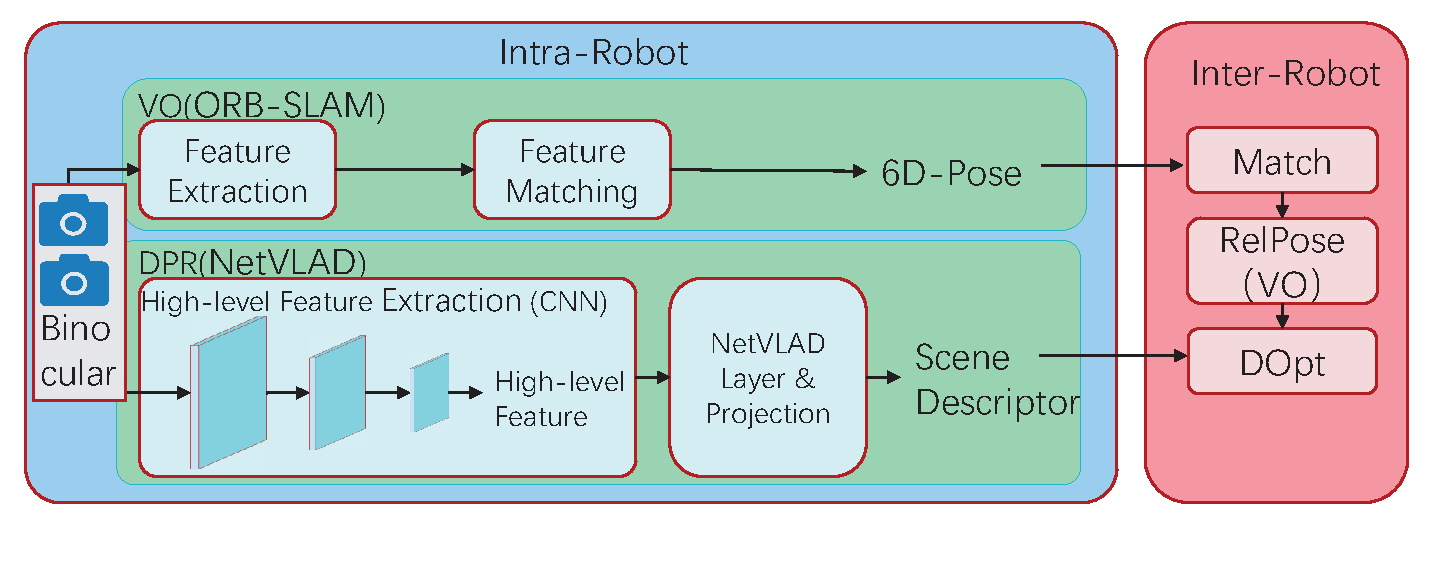
\includegraphics[width=1\textwidth]{fig/overview_pre.eps}\label{fig:all_pre}}
    \end{minipage}
    \begin{minipage}[t]{0.5\linewidth}  
    \centering  
    \subfigure[Our CNN-based DSLAM.] {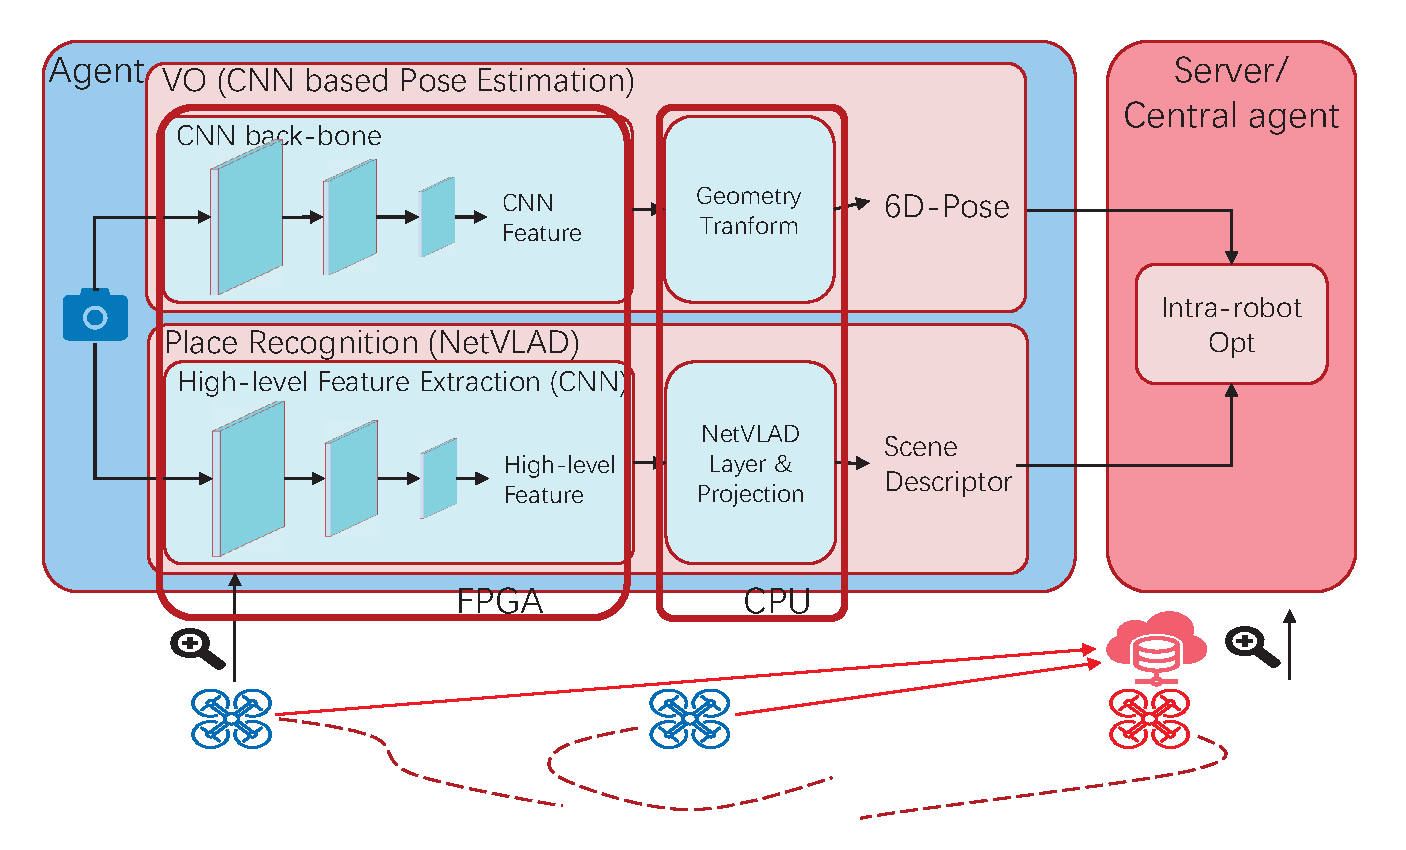
\includegraphics[width=1\linewidth]{fig/overview_us.eps}\label{fig:all_us}} 
    \end{minipage}
    \caption{(a) The previous work uses ORB feature-point based method to estimate the trajectory from the sequence of the stereo camera, and use NetVLAD \cite{Arandjelovic:2017997} to do DPR. (b) Our framework adopt Depth-VO-Feat \cite{Zhan:2018e92} in DSLAM system as the monocular VO, and we use the same method of NetVLAD in \cite{Cieslewski:20187ee} to do DPR. We use Xilinx Zynq MPSoC hardware platform to for deployment.
    }
\label{fig:overview}
\end{figure*}

Monocular systems are much easier to deploy than binocular systems. The transitional monocular feature point based VO should use complex depth reconstruction methods to compute the absolute scale of the pose scale\cite{pizzoli2014remode}, leading to speed-down. With the development of CNN, we can reconstruct the depth and pose with the absolute scale from the monocular camera directly, making monocular VO more robust and efficient\cite{Zhan:2018e92}. ecent advances in deep learning and the availability of large labelled visual datasets have significantly improved the accuracy of place recognition, such as NetVLAD\cite{Arandjelovic:2017997}. However, previous works concentrate on the accuracy of the CNNs, yet consider little about the deployment CNNs on the embedded system.

Though DSLAM system can benefit from the development of CNN, the fully CNN-based DSLAM system faces some key issues: 1) The embedded system usually support fixed-point CNN. 2) The speed will decline in the embedded system when running several CNN models simultaneously, the speed-down of DPR will lead to the decline of the final DSLAM accuracy. Therefore, we build up a CNN-based monocular DSLAM system on embedded FPGA platform, with following contributions:

\begin{itemize}
\item To the best of our knowledge, this work is the first to implement all components of monocular DSLAM with CNN.
% We adopt Depth-VO-Feat \cite{Zhan:2018e92} in DSLAM system to estimate the pose from the input monocular camera. We use the same method of NetVLAD in  \cite{Cieslewski:20187ee} to do place recognition. 
We deploy the system on Xilinx Zynq MPSoC hardware platform with DPU \cite{Tech:2019360}, which is an embedded CNN accelerator. The proposed DSLAM framework is illustrated in \cref{fig:all_us}.
\item As the embedded system usually support fixed-point CNN, we propose a pose-sensitive fixed-point fine-tune method to make the feature extraction layers fixed-point and remain the pose prediction layers floating-point, reaching the same accuracy with the original floating-point VO network. We schedule the fixed-point layers on DPU and the floating-point layers on CPU, so that we can accelerate the VO to 10ms.
\item The frequency of the NetVLAD influences the final result of DSLAM. We propose a cross-components scheduling method to scheduling the computation flow across VO and DPR, and pipeline the computation across the PL and PS of MPSoC to make full use of the embedded platform. We calculate the NetVLAD every 4 input frames from every 6 frames, improving the final accuracy of DSLAM. 
We also propose a new indicator called loop-closure recall (LCR), which indicates the remaining rate of loop-closure after trajectory merging, to evaluate the performance of trajectory merging. The output result of DSLAM with different NetVLAD frequency is illustrated in \cref{fig:dslamresult}. The tranditional average trajectory error (ATE) can not indicate the performance of trajectory merging in DSLAM.
\end{itemize}



\begin{figure}[thb]
    \begin{minipage}[t]{0.475\linewidth}  
    \centering
    \subfigure[NetVLAD/8 frames. \protect\          ATE=9] {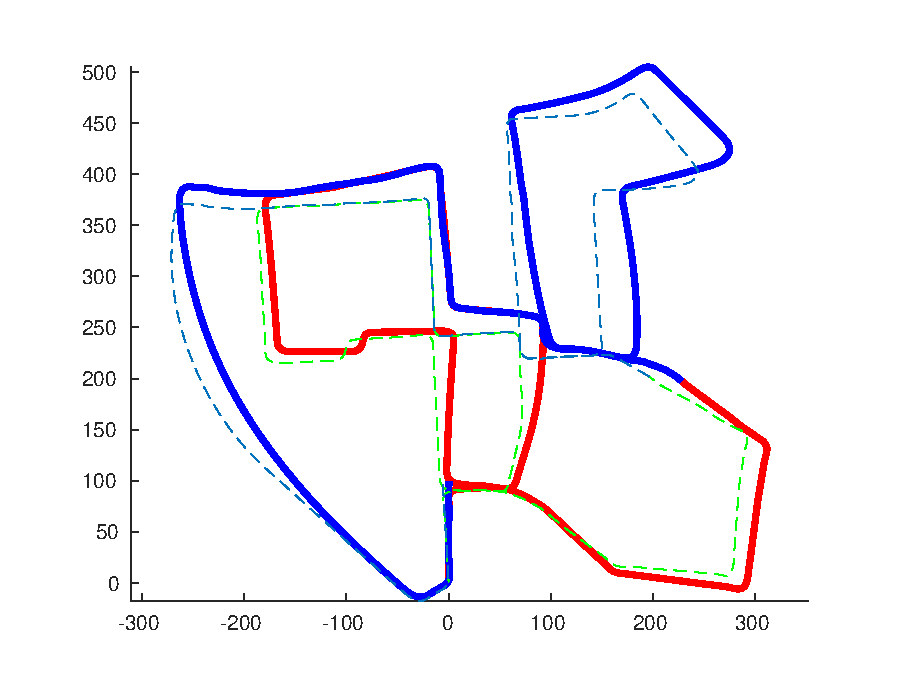
\includegraphics[width=1\linewidth]{fig/8netvlad.eps}\label{fig:8netvlad}}
    \end{minipage}
    \begin{minipage}[t]{0.475\linewidth}  
    \centering  
    \subfigure[NetVLAD/12 frames. \protect\ ATE=9] {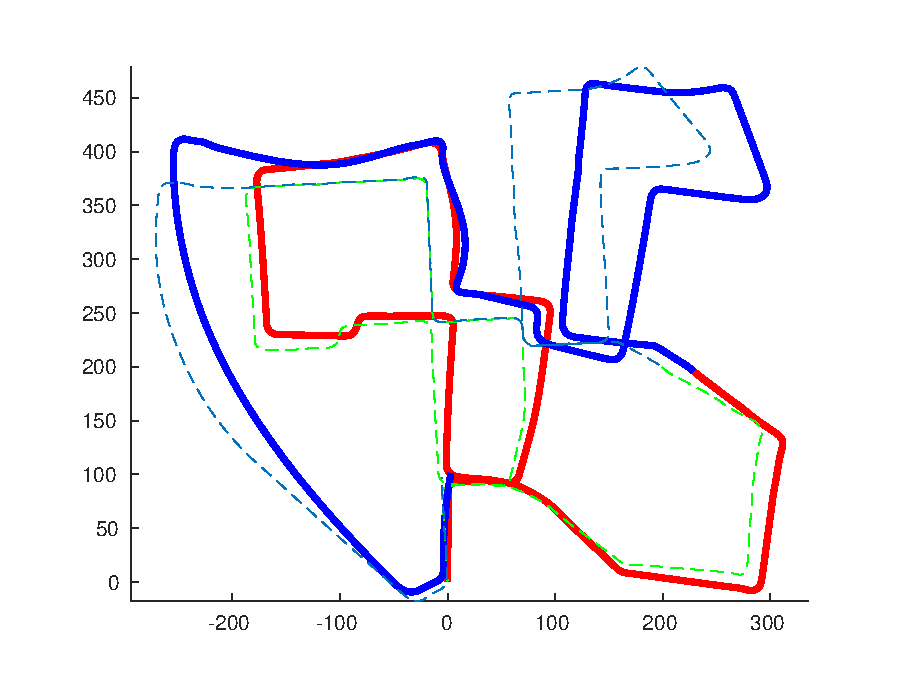
\includegraphics[width=1\linewidth]{fig/12netvlad.eps}\label{fig:12netvlad}} 
    \end{minipage}
    \caption{The DSLAM result of two robots(red and blue, the dashed is the ground truth the robots). (a) When do NetVLAD every 8 frames, the trajectories can be merged correctly. (b) When do NetVLAD every 12 frames, the trajectories can not be commendably merged. However, the ATE of these two results is similar.
    }
\label{fig:dslamresult}
\end{figure}



% The rest part of this article is orgnized as follows. \Cref{sec:background} will give the basic idea of CNN based methods and the hardware architecture of embedded platform, Xilinx Zynq MPSoC. \Cref{sec:hardsoft} will detail the implementation of our pose-sensitive fixed-point fine-tune method and the cross-components scheduling method. The experiment results will be given in \Cref{sec:experiment}. \Cref{sec:conclusion} will conclude this paper.

\section{Background and Motivation}
\label{sec:background}
\subsection{CNN based methods in DSLAM}
As described before, there are two essential components on each agent: 1) Visual Odometr(VO) and 2) Place Recognition.

\subsection{Hardware architecture of Zync SoC}
The Xilinx Zync Soc is a chip with ARM cores and FPGA fabric.


\section{Hardware-Software Co-design DSLAM}
\label{sec:hardsoft}
Our hardware-software co-design DSLAM system contains two essential improvements in the pose estimation and place recognition tasks. As illustrate in \cref{fig:all_us}, both of these two components are divided into two stages: $1)$ CNN front end to extract features which is deployed to the DPU on PL and $2)$ geometric operations to present final results which are deployed on the PS ARM cores. To make full use of the Zynq MPSoC (illustrated in \cref{fig:plps}), we optimize the data follow for both of these components.

\begin{figure}[t]  
    \centering  
    {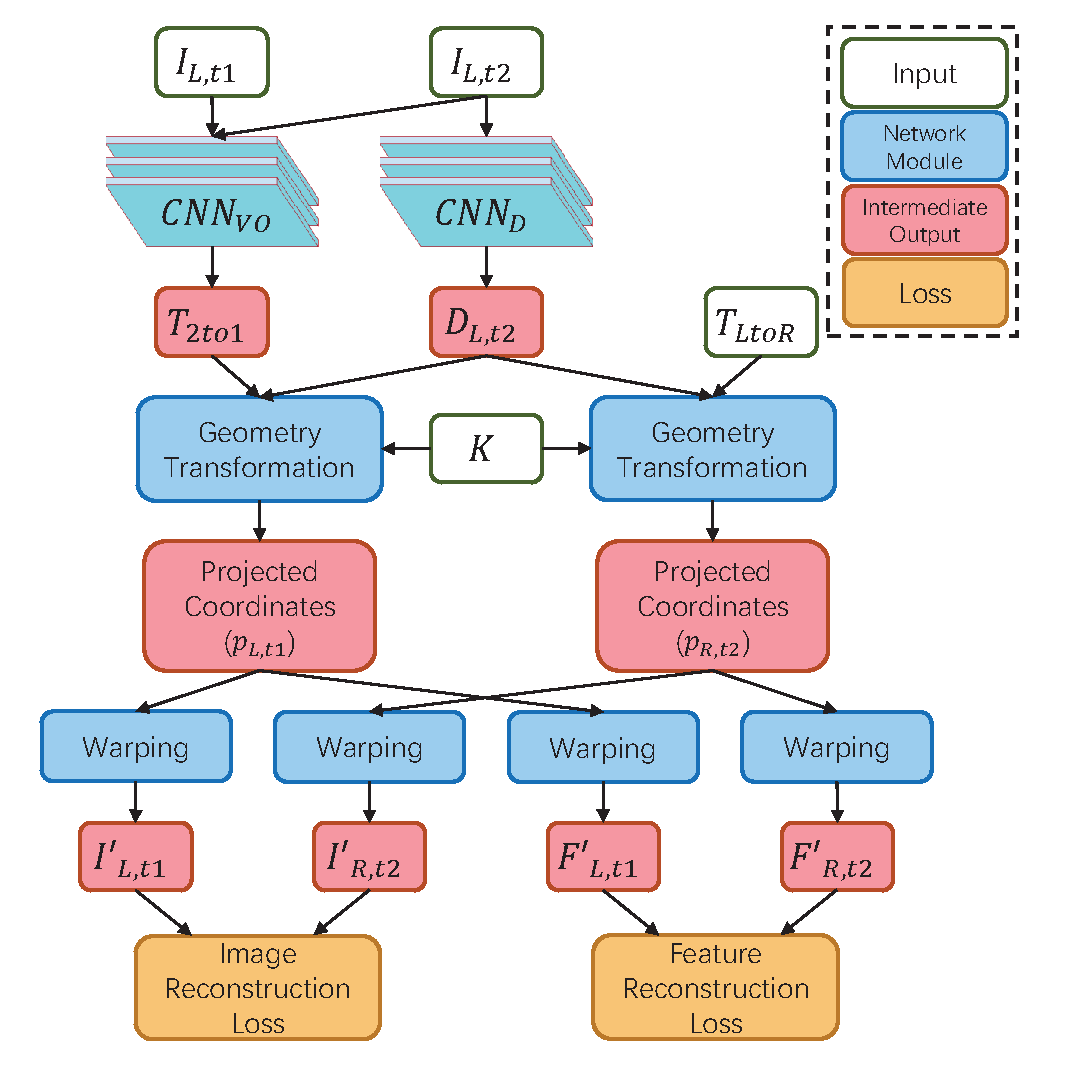
\includegraphics[width=0.85\linewidth]{fig/depth_vo_feat.eps}\label{fig:dvo}}
    \caption{Illustration of Depth-VO-Feat framework in the training phase, where $T_{LtoR}$ is the relative camera pose transformations between right and left views, and $K$ denotes the known camera intrinsic matrix. $CNN_{VO}$ and $CNN_D$ are convolutional nets for visual odometry and depth estimation respectively, which can be used independently in the testing phase. }
\end{figure}

\subsection{Pose Estimation}
We adopt Depth-VO-Feat \cite{Zhan:2018e92} in DSLAM system to estimate the pose from the input monocular camera. Monocular visual SLAM is a key issue in the field of robotics, while there are two challenging problems: $1)$ it is difficult and expensive to obtain accurate labeled data, $2)$ the methods that use monocular sequences in training always suffer from the scale-ambiguity problem, i.e., the actual scale of translations is missing, and only the direction is learned. In Depth-VO-Feat \cite{Zhan:2018e92}, we use image reconstruction loss as a self-supervised signal to train the convolutional neural networks and jointly train two networks for depth and odometry estimation without external supervision, which can be used independently in the testing phase. Besides, to fix this scale-ambiguity issue, we use stereo sequences in the training phase and monocular sequences in the testing phase. With the known spatial relationship between the left and right cameras, our neural networks can learn the real world scale. Feature reconstruction loss is an additional supervision signal, used to improve the robustness of this framework. Moreover, we use depth smoothness loss to encourage the predicted depth to be smooth, which demonstrated success in prior works. Then the final loss becomes:

\begin{equation}
    L=\lambda_{ir}L_{ir}+\lambda_{fr}L_{fr}+\lambda_{ds}L_{ds}
    \label{equ:loss}
\end{equation}

where $L_{ir}$, $L_{fr}$ and $L_{ds}$ are image reconstruction loss, feature reconstruction loss and depth smoothness loss respectively, $\lambda_{ir}$, $\lambda_{fr}$ and $\lambda_{ds}$ are the loss weightings for each loss term. The training framework is illustrated in \cref{fig:dvo}.


In order to run Depth-VO-Feat efficiently on the FPGA platform, we use fixed-point arithmetic units in the hardware to replace the floating-point number format in GPU and CPU. Many previous works have shown that 8-bit quantization for weights and featuremaps can make the networks run faster on FGPA. Here we adopt the fixed-point finetune method in \cite{Yu:2018:IDC:3299999.3283452}, in that we use the fixed-point number representation in the feed forward phase and keep floating-point number representation for backpropagation, and both weights and data will be re-quantized after each backpropagation. The fixed-point method will lead to a slight accuracy loss of the model, and the performance of the fixed-finetuned Depth-VO-Feat will be shown in detail in \cref{sec:experiment}.

% As the fixed-point method will lead to the accuracy loss of the model, we attempt several different quantization strategies to balance speed and accuracy, which will be shown in detail in \cref{sec:experiment}.

\subsection{Place Recognition}

\begin{figure}[t]
    \centering  
    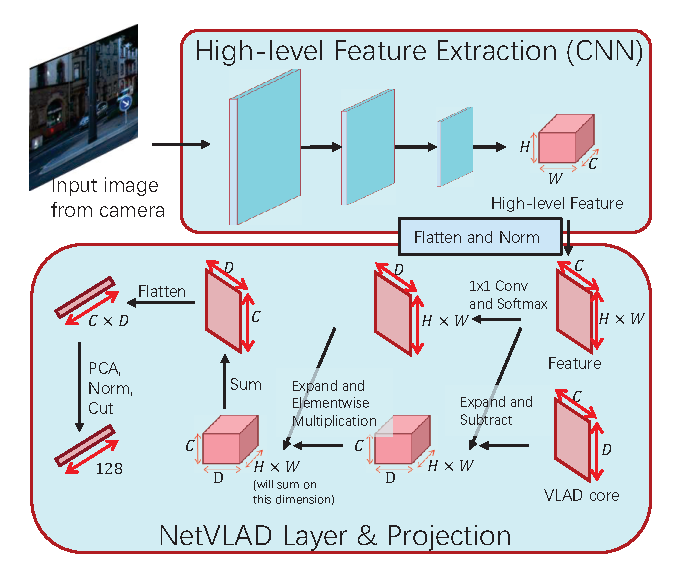
\includegraphics[width=0.95\linewidth]{fig/NetVLAD.eps}
    \caption{Process of NetVLAD. The CNN encoder is running at the CNN acclerator on PL side, and the VLAD layer as well as the PCA is running at the ARM core at PS side.}
    \label{fig:NetVLAD}
\end{figure}

The place recognition method provide the encoded vector transferred to the central agent for inter-robot place matching. As described in \cref{sec:background}, CNN has achieved significant improvements in place recognition tasks, and NetVLAD \cite{Arandjelovic:2017997} is one of the most impressive methods. The computation flow of NetVLAD is illustrated in \cref{fig:NetVLAD}. The CNN-based place recognition methods give the global descriptor of a camera frame in a two-step manner: $1)$ Firstly, a CNN encoder fetches the high-level feature map. $2)$ A vectorization component that aggregates the feature map into a shot global descriptor. The VLAD layer \cite{Arandjelovic:2017997} is a recently proposed plug-and-play operation that greatly improves the performance of place recognition. In the original work with the VLAD layer \cite{Arandjelovic:2017997}, the feature extraction encoder is a typical CNN named VGG-16 \cite{Simonyan:20143be}. The output dimension of original NetVLAD is usually tens of thousands, which is very difficult to be stored on the embedded system, not to mention in the communication-constrained environment. The PCA and the projection method can drastically reduce the output dimension. The previous works\cite{Cieslewski:20187ee} show that 128 dimension is plenty for DSLAM. The data flow and operations of the NetVLAD layer and the projection are complex and require the floating-point number, which cannot be supported with Deephi DPU. We implement the NetVLAD layer and the projection on the PS side of Zynq MPSoC.


Unlike the fixed-point finetune method used for pose estimation. The training procedure with huge non-public datasets is very complicated, and also we cannot finetune the NetVLAD model because of the lack of training data. We simply analyze the dynamic range of the weight and intermediate feature map of each CNN layer and figure out the optimal decimal point position for each layer respectively to minimize the truncation error of each layer.
This method is proposed in \cite{Qiu:2016151} and is used in many tasks such as image classification and image detection.

\subsection{Parallel Scheduling for VO and NetVLAD}

The time consumption of NetVLAD and VO is imbalanced. We do pipeline optimization to schedule the two components on Zynq MPSoC efficiently. The pipeline is illustrated in \cref{fig:pipline}. The interval time for reading camera is $T_{f}$. The CNN time for NetVLAD and VO is $T_{0}$ and $T_{1}$. The computation time cost on PS for VO and NetVLAD is $T_{2}$ and $T_{3}$. We do VO every input frame and do NetVLAD every $N$ frames.

\begin{figure}[t]
    \centering  
    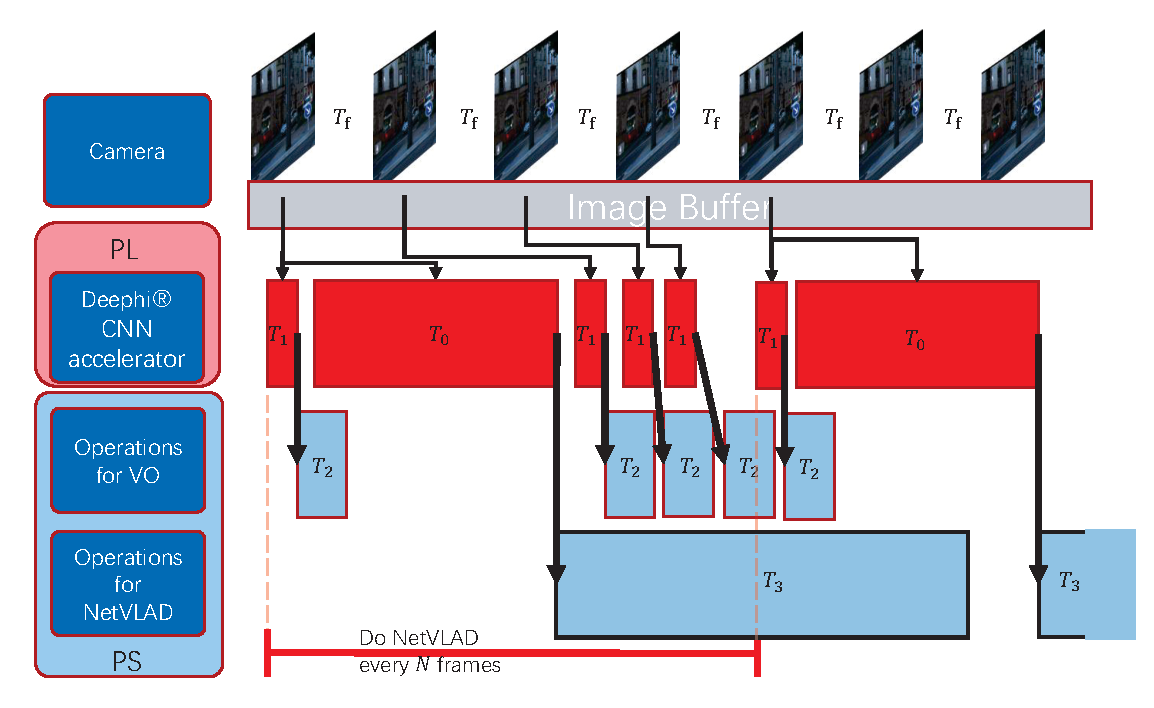
\includegraphics[width=0.95\linewidth]{fig/pipeline.eps}
    \caption{Scheduling pipeline. There are four threads: Camera read, Deephi core at PL, PS Operations for VO, and PS Operations for NetVLAD.}
    \label{fig:pipline}
\end{figure}

% The constrain of these computation time and $N$ is given as \cref{equ:pipline}.

Considering the thread on PL, the time constraint is given as \cref{equ:pipeline1}. 

\begin{equation}
    N \times T_{f} > T_{0} + N \times T_{1}
    \label{equ:pipeline1}
\end{equation}

The thread for VO on PS constrains the NetVLAD frequency as \cref{equ:pipeline2}.

\begin{equation}
    N \times T_{f} > T_{0} + T_{1} + (N-1) \times T_{2}
    \label{equ:pipeline2}
\end{equation}

The PS part of NetVLAD should finish before computing the PS part of next NetVLAD frame. This constraint can be written as \cref{equ:pipeline3}.

% The PS part of NetVLAD should finish before computing the PS part for next NetVLAD frame, and can be writen as \cref{equ:pipline3}.

\begin{equation}
    N \times T_{f} > T_{3}
    \label{equ:pipeline3}
\end{equation}

The execution time of our design will be given in \cref{sec:experiment}.


\section{Experiments}
\label{sec:experiment}
The experiment results shows our proposed DSLAM system can perform in real time and achieves similar accuracy with previous work.

\section{Conclusion}
\label{sec:conclusion} 

Though DSLAM can benefit from CNN, the deployment of CNN on embedded systems faces big challenges. We propose a CNN-based monocular DSLAM system deployed on Xilinx ZU9 MPSoC, and a Pose-Sensitive fixed-point finetune method to balance the accuracy and speed of CNN-based Visual Odometry on embedded FPGA. We also explore the impact of NetVLAD frequency on DSLAM results, and propose a cross-component scheduling method to increase the operating frequency of NetVLAD to improve DSLAM performance.


\section*{Acknowledgment}
This work was supported by National Natural Science Foundation of China (Grant No.61874156)


\bibliographystyle{IEEEtran}
\bibliography{src/fpgaslam}

\end{document}
